%% fig_product.tex -- multiplicativity of the Weil class, and the loci it
%% reaches inside the family.  Left: the K-line of each factor and of the
%% product, drawn as a tower.  Right: dimensions of the known loci against the
%% dimension of the family.
\documentclass[tikz,border=9pt]{standalone}
\usepackage{amsmath,amssymb}
\usetikzlibrary{arrows.meta,calc,backgrounds,positioning}
%% palette.tex -- shared colour definitions for the figures
\definecolor{PInk}{RGB}{26,32,44}
\definecolor{PBlue}{RGB}{37,82,139}
\definecolor{PTeal}{RGB}{23,127,125}
\definecolor{POchre}{RGB}{193,138,44}
\definecolor{PClay}{RGB}{178,74,58}
\definecolor{PSlate}{RGB}{108,122,137}
\definecolor{PViolet}{RGB}{110,86,150}
\definecolor{WBlue}{RGB}{223,234,246}
\definecolor{WTeal}{RGB}{220,238,236}
\definecolor{WOchre}{RGB}{250,240,218}
\definecolor{WClay}{RGB}{247,229,224}
\definecolor{WSlate}{RGB}{238,241,244}
\definecolor{PMag}{RGB}{158,58,110}
\definecolor{PGrass}{RGB}{62,124,66}
\definecolor{PAmber}{RGB}{214,112,38}
\definecolor{PIndigo}{RGB}{58,64,140}
\definecolor{PRule}{RGB}{176,186,197}

%% shared macros so the standalone figures match the paper
\providecommand{\QQ}{\mathbb{Q}}
\providecommand{\ZZ}{\mathbb{Z}}
\providecommand{\RR}{\mathbb{R}}
\providecommand{\CC}{\mathbb{C}}
\providecommand{\PP}{\mathbb{P}}
\providecommand{\Kx}{K^{\times}}
\providecommand{\HW}{W}
\providecommand{\Nm}{\mathrm{N}}
\providecommand{\Hdg}{\mathrm{Hdg}}
\providecommand{\NS}{\mathrm{NS}}
\providecommand{\cA}{\mathcal{A}}
\providecommand{\cD}{\mathcal{D}}
\providecommand{\cF}{\mathcal{F}}
\providecommand{\cP}{\mathcal{P}}
\providecommand{\cO}{\mathcal{O}}
\providecommand{\cQ}{\mathcal{Q}}
\providecommand{\bbar}[1]{\overline{#1}}
\providecommand{\ch}{\operatorname{ch}}
\providecommand{\End}{\mathrm{End}}


\tikzset{obl/.style={x={(1cm,0cm)}, y={(0.52cm,0.40cm)}, z={(0cm,1cm)}}}

%% a thin K-line plate: corner (x0,y0,z0), width w, depth p, thickness t
\newcommand{\plate}[7]{%
  \begin{scope}[obl]
    \fill[#7 top] (#1,#2,#3+#6) -- (#1+#4,#2,#3+#6) -- (#1+#4,#2+#5,#3+#6) -- (#1,#2+#5,#3+#6) -- cycle;
    \fill[#7 front] (#1,#2,#3) -- (#1+#4,#2,#3) -- (#1+#4,#2,#3+#6) -- (#1,#2,#3+#6) -- cycle;
    \fill[#7 side] (#1+#4,#2,#3) -- (#1+#4,#2+#5,#3) -- (#1+#4,#2+#5,#3+#6) -- (#1+#4,#2,#3+#6) -- cycle;
    \draw[#7 edge] (#1,#2,#3) -- (#1+#4,#2,#3) -- (#1+#4,#2,#3+#6) -- (#1,#2,#3+#6) -- cycle;
    \draw[#7 edge] (#1+#4,#2,#3) -- (#1+#4,#2+#5,#3) -- (#1+#4,#2+#5,#3+#6) -- (#1+#4,#2,#3+#6);
    \draw[#7 edge] (#1,#2,#3+#6) -- (#1,#2+#5,#3+#6) -- (#1+#4,#2+#5,#3+#6);
  \end{scope}}

\tikzset{
  f top/.style={fill=WTeal}, f front/.style={fill=WTeal!78!PTeal!35},
  f side/.style={fill=WTeal!58!PTeal!45}, f edge/.style={draw=PTeal,line width=0.6pt},
  p top/.style={fill=WOchre}, p front/.style={fill=WOchre!78!POchre!35},
  p side/.style={fill=WOchre!58!POchre!45}, p edge/.style={draw=POchre,line width=0.8pt},
}

\begin{document}
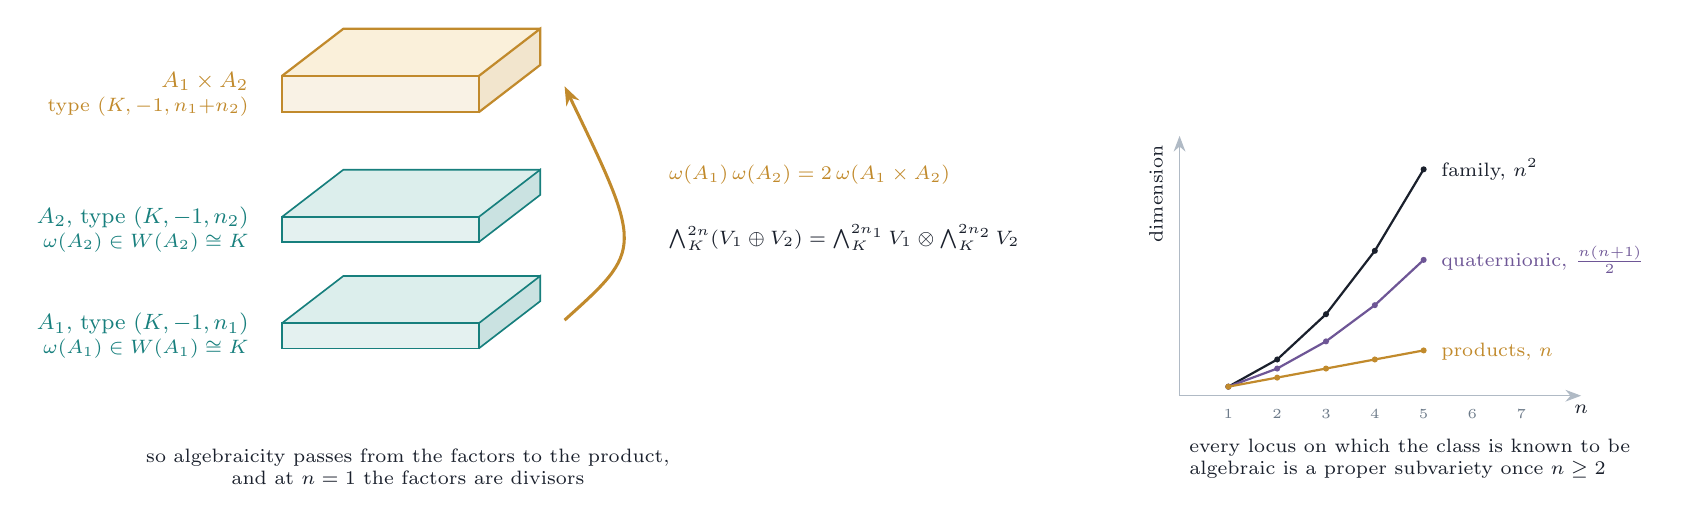
\begin{tikzpicture}[font=\footnotesize,text=PInk]

%% =====================================================================
%% Left panel: the two factors and the product.
%% =====================================================================
\begin{scope}
  \plate{0}{0}{0}{2.5}{1.5}{0.32}{f}
  \begin{scope}[obl]\coordinate (F1) at (0,0,0.16);\coordinate (F1r) at (2.5,0.75,0.16);\end{scope}
  \node[anchor=east,align=right,text=PTeal] at ([xshift=-3mm]F1)
    {$A_{1}$, type $(K,-1,n_{1})$\\[-1pt]{\scriptsize $\omega(A_{1})\in\HW(A_{1})\cong K$}};

  \plate{0}{0}{1.35}{2.5}{1.5}{0.32}{f}
  \begin{scope}[obl]\coordinate (F2) at (0,0,1.51);\coordinate (F2r) at (2.5,0.75,1.51);\end{scope}
  \node[anchor=east,align=right,text=PTeal] at ([xshift=-3mm]F2)
    {$A_{2}$, type $(K,-1,n_{2})$\\[-1pt]{\scriptsize $\omega(A_{2})\in\HW(A_{2})\cong K$}};

  \plate{0}{0}{3.0}{2.5}{1.5}{0.46}{p}
  \begin{scope}[obl]\coordinate (P) at (0,0,3.23);\coordinate (Pr) at (2.5,0.75,3.23);\end{scope}
  \node[anchor=east,align=right,text=POchre] at ([xshift=-3mm]P)
    {$A_{1}\times A_{2}$\\[-1pt]{\scriptsize type $(K,-1,n_{1}{+}n_{2})$}};

  % the multiplication arrow up the right-hand side
  \draw[-{Stealth[length=2.4mm]},POchre,line width=1.1pt]
    ([xshift=7mm,yshift=-1mm]F1r) .. controls ([xshift=17mm,yshift=8mm]F1r) ..
    ([xshift=7mm,yshift=-2mm]Pr);
  \node[anchor=west,align=left,text=POchre,font=\scriptsize] at ([xshift=19mm,yshift=4mm]F2r)
    {$\omega(A_{1})\,\omega(A_{2})=2\,\omega(A_{1}\times A_{2})$};
  \node[anchor=west,align=left,text=PInk,font=\scriptsize] at ([xshift=19mm,yshift=-4mm]F2r)
    {$\bigwedge^{2n}_{K}(V_{1}\oplus V_{2})
      =\bigwedge^{2n_{1}}_{K}V_{1}\otimes\bigwedge^{2n_{2}}_{K}V_{2}$};

  \node[anchor=north,align=center,font=\scriptsize,text=PInk] at (1.6,-1.15)
    {so algebraicity passes from the factors to the product,\\
     and at $n=1$ the factors are divisors};
\end{scope}

%% =====================================================================
%% Right panel: dimensions of the loci reached, against the family.
%% =====================================================================
\begin{scope}[shift={(11.4,-0.6)}]
  \def\ux{0.62}   % x unit per n
  \def\uy{0.115}  % y unit per dimension
  \draw[PRule,-{Stealth[length=2mm]}] (0,0) -- (5.1,0) node[anchor=north,font=\scriptsize,text=PInk] {$n$};
  \draw[PRule,-{Stealth[length=2mm]}] (0,0) -- (0,3.3) node[anchor=east,font=\scriptsize,text=PInk,rotate=90,yshift=3mm] {dimension};
  \foreach \n in {1,2,3,4,5,6,7}
    \node[font=\tiny,text=PSlate,anchor=north] at (\n*\ux,-0.05) {\n};

  % family n^2
  \draw[PInk,thick] plot coordinates {(1*\ux,1*\uy) (2*\ux,4*\uy) (3*\ux,9*\uy) (4*\ux,16*\uy) (5*\ux,25*\uy)};
  \foreach \n/\v in {1/1,2/4,3/9,4/16,5/25} \fill[PInk] (\n*\ux,\v*\uy) circle (1.1pt);
  \node[anchor=west,font=\scriptsize,text=PInk] at (5*\ux+0.1,25*\uy) {family, $n^{2}$};

  % quaternionic n(n+1)/2
  \draw[PViolet,thick] plot coordinates {(1*\ux,1*\uy) (2*\ux,3*\uy) (3*\ux,6*\uy) (4*\ux,10*\uy) (5*\ux,15*\uy)};
  \foreach \n/\v in {1/1,2/3,3/6,4/10,5/15} \fill[PViolet] (\n*\ux,\v*\uy) circle (1.1pt);
  \node[anchor=west,font=\scriptsize,text=PViolet] at (5*\ux+0.1,15*\uy) {quaternionic, $\tfrac{n(n+1)}{2}$};

  % product locus n
  \draw[POchre,thick] plot coordinates {(1*\ux,1*\uy) (2*\ux,2*\uy) (3*\ux,3*\uy) (4*\ux,4*\uy) (5*\ux,5*\uy)};
  \foreach \n/\v in {1/1,2/2,3/3,4/4,5/5} \fill[POchre] (\n*\ux,\v*\uy) circle (1.1pt);
  \node[anchor=west,font=\scriptsize,text=POchre] at (5*\ux+0.1,5*\uy-0.02) {products, $n$};

  \node[anchor=north west,align=left,font=\scriptsize,text=PInk] at (0,-0.42)
    {every locus on which the class is known to be\\
     algebraic is a proper subvariety once $n\ge2$};
\end{scope}

\end{tikzpicture}
\end{document}
